% Chapter Template

\chapter{Data gathering and preprocessing}
\label{Chapter2}
Data was sourced from several streams. The Icelandic Meterological Office (IMO) provided measurements from weather stations all around Iceland. NWP data was downloaded from Copernicus Arctic Regional Reanalysis dataset (CARRA). A land elevation model was also provided by IMO.

\section{Automatic Weather Station Data}

IMO provided 10 minute measurements from \nStationsMin weather stations all around Iceland. The measurements that met the filtering criteria, started in \startDateVedur and ended in 2023. Of these \nStationsMin stations, \nVedurMin were from IMO and placed at 10 meters above ground, while the rest (\nVGMin) were from \href{https://www.vegagerdin.is/}{the Icelandic Road and Coastal Administration (IRCA)} and placed at 6-7 meters above ground\cite{vegagerdin_postur}. The location of these weather stations can be seen in Figure \ref{fig:aws_map}. The information that is provided by these Automatic Weather Stations (AWS) is presented in two different types of data files, hourly and 10 minute files. The hourly files are summations of the 10 minute files, with the exception that errors, such as nails, still in the 10 minute files should have been removed from the hourly documents. Nails, are sharp increases from the rest of the data and are unrealistic outliers that are considered measurement errors and are discarded. Each type of document contain the following information: the date and time, the station number (that can be converted to the coordinates using another data set), the average wind speed ($f$), the wind gust ($f_g$), the standard deviation of the wind gust, the direction of the wind ($d$) and the standard deviation for the wind direction. These measurement started at the end of the 20th century, when the first AWS stations was installed. More have been added in the following decades. This thesis does not look at the data as a time series, it tries to make predictions using only the information at a given point in time.

\begin{figure}
    \centering
    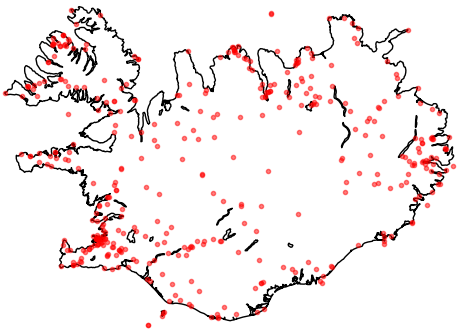
\includegraphics[scale = 1]{Figures/stationsOverIceland_2024-05-16_stripped_to_frame.png}
    \caption[Locations of automatic weather stations in Iceland]{Locations of all 412 stations that were looked at in this study. Most of these were from IMO but over a hundred were from IRCA. IMO AWS are placed at 10 meters above ground, while IRCA stations are placed at around 6-7 meters above ground.}
    \label{fig:aws_map}
\end{figure}

\section{CARRA Data}
The CARRA dataset goes back to September 1991 and is currently updated monthly, with a latency of 2-3 months\cite{carra_information}. The oldest IMO data point that fulfills given criteria is from \startDateVedur. This is covered by CARRA. The CARRA dataset is available for two regions, West and East. Each of these covers a vastly larger area than the area of interest. This leads to having to store a large amount of data. To get the data one has two options. Their web interface or using their API client. Using the API client is the only realistic option here, as there were thousands of requests made for different times. If using the API, it is possible to query a smaller area (such as a rectangular area around Iceland) given a set of coordinates.

The requests to the API are made at each available CARRA hour ([00, 03, 06, 09, 12, 15, 18, 21]) for each available observation. Only these hours can be used as the CARRA predicted output is represents the wind speed at those given hours and would thus not encapsulate well the extreme values in between these times. Using these datapoints, interpolation was used to get an estimation for the point of the given weather station. The CARRA data contains several types of layers. These are single levels, model levels, height levels, pressure levels. The data for this thesis was downloaded from height levels. That is, data was requested at heights of 15, 250 and 500 meters above ground. For each point 4 parameters were requested, wind speed, wind direction, pressure and temperature. Each of these features needed to be interpolated to create data for model to be trained on.

\section{Elevation data}
IMO provided a TIFF file containing the elevation of Iceland on a 20 meter by 20 meter grid. This file encompasses Iceland and is around 685 MB. A good amount of time was spent finding a data structure that was best for lookup when trying to find points within a certain area. The country was divided into 10 parts (as only around 13\% of the file was able to be read into memory at each time as a part of dictionary object) with boundary boxes. The Python package Rasterio allowed for quick lookup with it's index and the affine transform. Using this package it is possible to quickly look up elevation given coordinates using matrix calculations.